The main characteristic of images which lead the traditional algorithm of encryption to not be adapted to image encryption is the correlation between adjacent pixels. \\
In order to quantify this phenomenon, we're going to display correlation diagram : random pixels are chosen in the image data, the value of this pixel is displayed on the X-axis, on the Y-axis is displayed the value of the adjacent pixel.

Moreover, the correlation coefficient of 2D variables can be computed following the equation :

\begin{equation*}
	r = \dfrac{cov(x,y)}{\sqrt{D(x)D(y)}}
\end{equation*}

where,
\vspace{-0.5em}
\begin{equation*}
	D(l) = \frac{1}{N} \sum_{i=1}^N \left(l_i - \frac{1}{N} \sum_{k=1}^N l_k \right)^2, \text{ with } l=x \text{ or } l=y
\end{equation*}

and, 
\vspace{-0.5em}
\begin{equation*}
	cov(x,y) = \frac{1}{N} \sum_{i=1}^N \left(x_i - \frac{1}{N} \sum_{k=1}^N x_k \right)  \left(y_i - \frac{1}{N} \sum_{k=1}^N y_k \right)
\end{equation*}


\begin{figure}[!h]
\centering
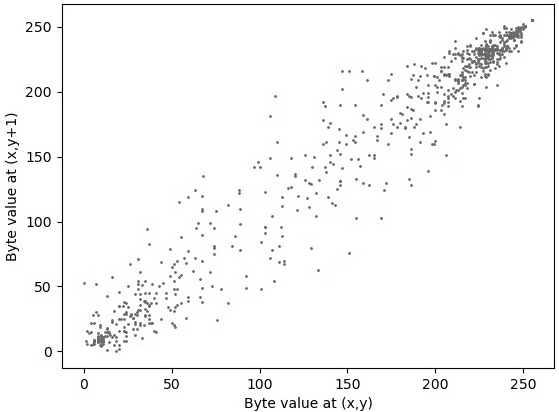
\includegraphics[scale=0.5]{tex/img/corregal.jpg}
\caption{Correlation diagram ($r = 0.981564$) for 1000 randomly chosen points of the original image \textit{galois.bmp}}
\end{figure}

To be considered as a good image encryption algorithm, the correlation diagram should not contain discernable patters and the correlation coefficient should be close enough to 0. 
\begin{figure}[!h]
\centering
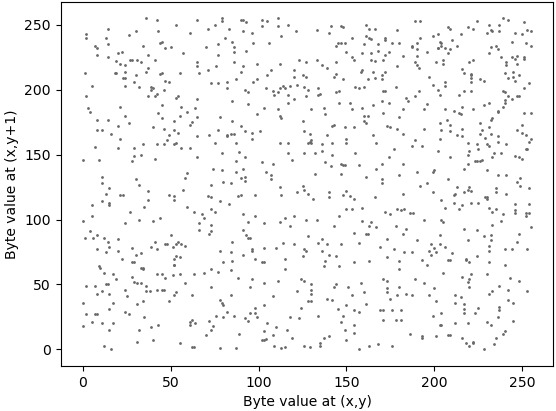
\includegraphics[scale=0.5]{tex/img/correegal.jpg}
\caption{Correlation diagram ($r = 0.083521$) for 1000 randomly chosen points of the encrypted image \textit{galois.bmp} with a XOR key of two logistic maps ($\mu_1=3.89$, $r_{01}=0.6104$) and ($\mu_2=3.79$, $r_{02}=0.902$)} 
\end{figure}

We can observe on \textit{Figure 7} that the correlation diagram of the encrypted image, with the proposed algorithm and the discrete logistic map, validate the requirement cited above. The proposed algorithm can be considered as a good encryption algorithm regarding the correlation of adjacent pixels analysis. 
